\chapter{Web-Tools für das Mikado-Projekt}
\label{ch:webtools}

Nach meiner Arbeit am IVS, Jira und Confluence wurde ich nun Teil eines anderen
Projekts namens Mikado\footnote{\url{http://www.mikado-robotics.de}}. Mikado ist ein Robotikprojekt,
bei dem es hauptsächlich um das sogenannte ``Bin Picking'' geht. Dabei wird ein
Roboter dazu eingesetzt, zufällig in einer Kiste liegende Teile mithilfe einer 3D-Kamera
zu erkennen, zu greifen und in eine andere Position zu bringen. Die Herausforderung
liegt hierbei beim Leeren der Kiste, d.h. alle sich darin befindlichen Teile gleichgültig
ihrer Position greifen zu können.

\begin{figure}[H]
	\begin{center}
		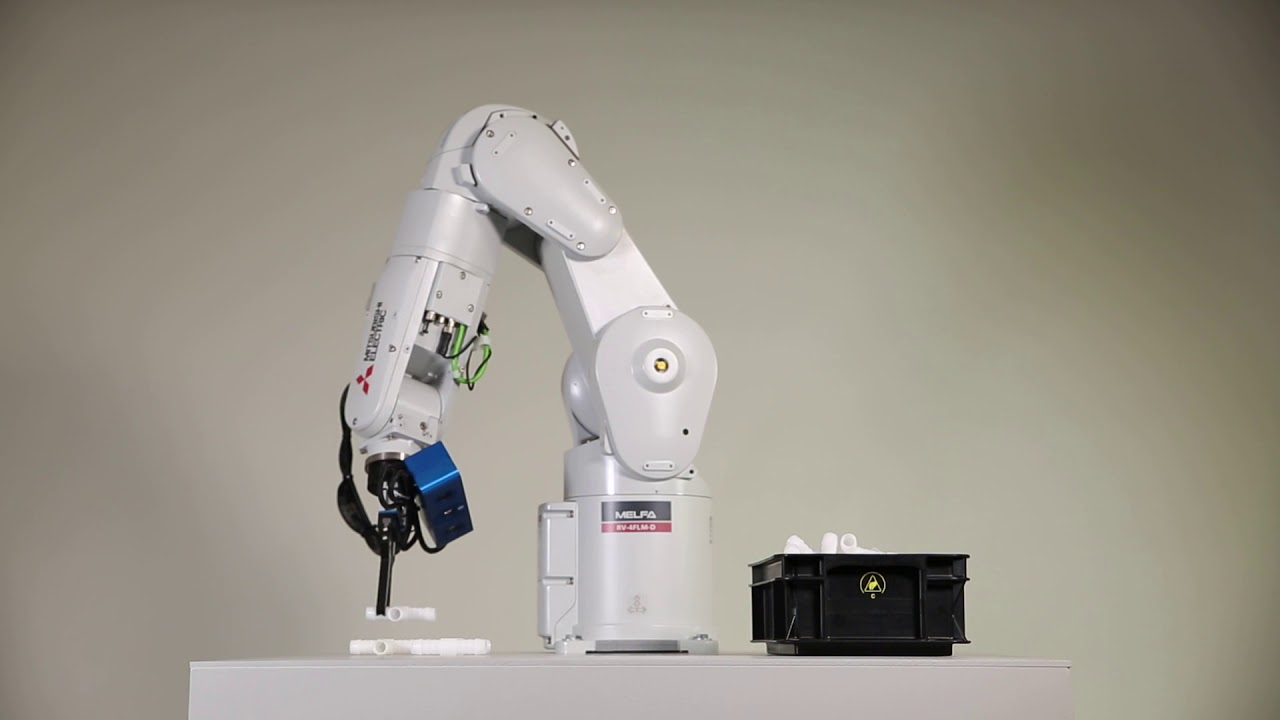
\includegraphics[width=0.75\textwidth]{media/mikado-roboter.jpg}
		\caption{Mikado-Roboter von Mitsubishi}
		\label{fig:mikado-roboter}
	\end{center}
\end{figure}



\section{Demoablauf für Messen}

Zum Kennenlernen der Programmschnittstelle und des Roboters sollte ich zunächst
mit dem von isys geschriebenen Programm einen Demoablauf aufbauen, welcher für
Messen oder ähnliche Anwendungsfälle verwendet werden sollte. Im Programm lassen
sich dafür Abläufe graphisch regeln, beispielsweise eine Bewegung, das Greifen
eines Teils oder die Bildaufnahme mit der 3D-Kamera. Diese noch nicht veröffentlichte
Software konnte somit außerdem von mir getestet und Verbesserungsvorschläge geäußert
werden.

Zur Erkennung der Teile wird mithilfe der Kameras ein 3D-Bild aufgenommen, welches
anschließend von der Recheneinheit analysiert und zu einer Punktwolke transformiert
wird. Diese Punktwolke wird nun mit dem eintrainierten CAD-Modell abgeglichen und
somit mögliche Kandidaten anhand ihrer Übereinstimmung identifiziert. Die dabei
gewählte Mindestübereinstimmung lässt sich dabei einstellen, was je nach Wert
Vor- bzw. Nachteile mit sich bringt:

\begin{table}[H]
	\begin{tabular}{| l || l |}
	\hline
	\textbf{Höhere Mindestqualität} & \textbf{ Niedrigere Mindestqualität}\\
	\hline\hline
	Erkannte Teile können mit höherer Sicherheit & Erkannte Teile können sich in nahezu un-\\
	richtig und sicher gegriffen werden & greifbarem Winkel befinden und daher nicht\\
	& sicher gegriffen werden\\
	\hline
	Weniger Teile werden erkannt, daher höhere & Viele Teile werden erkannt, die Wahrschein-\\
	Chance, die Kiste nicht leer zu bekommen & lichkeit ist daher größer, alle verbleibenden\\
	& Teile zu identifizieren\\
	\hline
	\end{tabular}
	\caption{Vor- bzw. Nachteile einer höheren vs. niedrigeren Mindestqualität}
	\label{mikado-demo-mindestqualität}
\end{table}

Die Bewegungen des Robotors lassen sich entweder über die Winkel der einzelnen Gelenke
(beim von isys verwendeten Roboter von Mitsubishi Electrics sind es 6 Gelenke) oder
das Format \texttt{xyz rpy} (\texttt{xyz} ist hierbei die Position im Raum (3 Koordinaten),
\texttt{rpy} (roll, pitch, yaw) die Drehung des Greifers) angeben. Sämtliche Bewegungen
und Rotationen sind dabei kollisionsgeprüft, d.h. sobald das System eine mögliche
Kollision erkennt, wird die Bewegung nicht ausgeführt. In diesem Fall kann eine
alternative Aktion durch einen Sprung im Programmablauf durchgeführt werden.

Über einzelne Sektionen und Sprünge lässt sich nun ein strukturiertes Programm erstellen,
was sowohl einfache Funktionen (wie in diesem Fall eine Demonstration der Funktionalität)
oder auch komplexe Abläufe wie den Zusammenbau eines Schneckengewindes übernehmen
kann. Der Programmablauf kann dabei mit den Funktionen \texttt{start}, \texttt{pause},
\texttt{step} und \texttt{reset} gesteuert werden, was in folgenden Aufgaben noch
wichtig wird.

Mein Demonstrationsprogramm war hierbei die Abwandlung einer älteren Demo. Der Roboter
nimmt dabei Zahnräder aus einer Kiste, testet mithilfe einer Lichtschranke, ob er
das Teil tatsächlich gegriffen hat, und legt dieses schlussendlich so ab, dass der
Schriftzug ``isys'' entsteht. Ist dies geschehen, nimmt er nacheinander die abgelegten
Teile wieder auf und legt sie zurück in die Kiste.

Der Zweck der Demonstration ist einerseits das Heranführen an den Roboter an sich
(z.B. die Arbeitsweise der Maschine oder die graphische Programmierung) sowie die
Fähigkeit, wirklich sämtliche Teile aus der Kiste nehmen zu können, zu demonstrieren.
Erreichen lässt sich dies einfach dadurch, dass zu Beginn nur so viele Zahnräder
in die Kiste gelegt werden, wie am Ende auch für den Schriftzug benötigt werden.



\section{Web-Remote für die Mikado-Software}

Für die Demonstration bei Messen oder bei ähnlichen Veranstaltungen sollte nun von
mir ein Webinterface erstellt werden, was als Fernzugriff für die Mikadosoftware
verwendet werden kann. Der Sinn dahinter ist, dass der Programmablauf nicht mehr
ausschließlich mithilfe von Bildschirm und Tastatur gesteuert, sondern beispielsweise
über ein Smartphone modern und komfortabel bedient werden soll. Dies ist insbesondere
nützlich, da aus Sicherheitsgründen bei Vorführungen eine Glaswand vor dem Roboteraufbau
ist, was Eingriffe in den Ablauf stark erschwert.


\subsection{Design der neuen Webseite}

Nachdem ich im \ref{ch:ivs}. Projekt bereits mit Javascript, CSS und HTML in Berührung
gekommen war, konnte ich nun eine völlig neue Webseite basierend auf meinen erlangten
Kenntnissen selbstständig und von Grund auf aufbauen. Dazu kümmerte ich mich zuerst
um Inhalt und Design der neuen Seite und fügte anschließend die Funktionalität durch
Javascript und jQuery hinzu.

\subsubsection{Struktur mit HTML}

Zunächst gliederte ich die neue Webseite mithilfe der zugehörigen HTML-Tags in sinnvolle
Abschnitte. Mit \texttt{<nav>}, \texttt{<main>} und \texttt{<footer>} sowie geschachtelten
\texttt{<div>}-Tags konnte ich eine sinnvolle Struktur in den Inhalt der Seite bringen.

Im \texttt{<nav>}-Teil der Seite wird die Navigationsleiste definiert; in meinem
Fall umfasste sie die Listenpunkte \textbf{Logs}, \textbf{Kontrolle} und \textbf{Über}
sowie ein \textbf{Hamburger-Menü-Icon}\footnote{\url{https://de.wikipedia.org/wiki/Hamburger-Men\%C3\%BC-Icon}},
welches zum Ein- und Ausklappen des Menüs notwendig war. Im \texttt{<main>}-Teil
des HTML-Dokuments wird sämtlicher Inhalt der Seite definiert, also in meinem Fall
das Logfenster, die Kontroll- und die Informationsseite. Diese einzelnen Abschnitte
sind jeweils wieder in einzelne \texttt{<div>}s geteilt, sodass Struktur und Design
gewährleistet werden können. Schlussendlich befinden sich im \texttt{<footer>}-Element
einige Informationen über das Produkt, wie z.B. Copyright, Webseite oder Kontakt.

\begin{code}[language=html, caption={Struktur der Kontrollseite}]
<div id="control" class="content">
	<div class="control-window">
		<div class="control-element">
			<button onclick="start()">
				<img src="media/start.svg" alt="Start">
			</button>
		</div>
		<div class="control-element">
			<button onclick="step()">
				<img src="media/step.svg" alt="Step">
			</button>
		</div>
		<div class="control-element">
			<button onclick="pause()">
				<img src="media/pause.svg" alt="Pause">
			</button>
		</div>
		<div class="control-element">
			<button onclick="reset()">
				<img src="media/reset.svg" alt="Reset">
			</button>
		</div>
	</div>
</div>
\end{code}

Wie man sieht, bestehen die Kontrollbuttons aus einem Funktionsaufruf (den ich erst
später implementiert habe) und einer SVG-Grafik\footnote{\url{https://de.wikipedia.org/wiki/Scalable\_Vector\_Graphics}}.

\subsubsection{Erstellen von SVG-Grafiken}

SVG-Grafiken haben den großen Vorteil, dass sie vom Browser gerendert werden. Dadurch
ist einerseits keine große Bilddatei notwendig, was (insbesondere auf mobilen Endgeräten)
zu sehr schnellen Ladezeiten führt, und andererseits auch nicht das Problem zu geringer
Auflösungen mit sich bringt, wodurch die Grafik immer gestochen scharf ist. Da jedoch
keine entsprechenden Grafiken vorhanden waren, musste ich diese selbst erstellen.
Auch für das Navigationsmenü habe ich SVG-Dateien entworfen.

Der Inhalt einer SVG-Grafik ist der Syntax von HTML bzw. XML sehr ähnlich. Zunächst
wird mit dem Tag \texttt{<svg>} gekennzeichnet, dass es sich um eine SVG-Grafik
handelt. Innerhalb dieses Tags können nun Bildelemente hinzugefügt werden:

\begin{code}[language=svg, caption={Bildelemente in einer SVG-Grafik}]
<svg width="54" height="54" viewBox="0 0 54 54" xmlns="http://www.w3.org/2000/svg" xmlns:xlink= "http://www.w3.org/1999/xlink">
	<circle
		cx="27" cy="27" r="25"
		stroke="black" stroke-width="4" fill="none"
	/>
	<line
		x1="18" y1="13"
		x2="18" y2="41"
		stroke="black" stroke-width="8" stroke-linecap="butt"
	/>
	<line
		x1="36" y1="13"
		x2="36" y2="41"
		stroke="black" stroke-width="8" stroke-linecap="butt"
	/>
</svg>
\end{code}

Hier wird beispielsweise zunächst ein umschließender Kreis definiert (ll. 2 - 5),
welcher den Mittelpunkt $P(27|27)$ und den Radius $r = 25$ hat. Die Linienfarbe
soll Schwarz sein, die Linienbreite 4 Pixel und der Kreis soll nicht gefüllt sein.
Anschließend werden zwei Linien gezeichnet, jeweils mit der Farbe Schwarz, der Breite
8px und einem geraden Linienende. Linie 1 geht in diesem Fall von $P(18|13)$ nach
$Q(18|41)$.

\subsubsection{Stilregeln durch CSS}

Im nächsten Schritt ging es um das Design mithilfe von CSS. Die vorhergehend definierten
Inhalte konnte ich nun schöner Darstellen, indem ich Stilregeln für bestimmte Elemente
und Klassen vornahm. Dazu gehörten unter Anderem die Schriftart, Farbschema für
Menüleiste und Links oder auch Positionierung von Abschnitten und Festlegen von
Abständen.

Sehr wichtig war hierbei die Orientierung an relativen Werten wie der Bildschirmweite
(\texttt{viewport width}). Da es sich hierbei um ein für Mobilgeräte optimiertes
Webinterface handelt, spielt Skalierbarkeit auf unterschiedliche Größen eine große
Rolle. Umsetzen lässt sich dies beispielsweise durch ein sogenanntes \textbf{Responsive
Design}\footnote{\url{https://de.wikipedia.org/wiki/Responsive_Webdesign}}, bei dem
die Webseite der Bildschirmgröße entsprechend reagiert. Dies sichert auch eine gute
und intuitive Darstellung beim Wechsel vom Portrait- in den Landschaftsmodus (z.B.
bei Tablet PCs).

In der Umsetzung erfolgt dies durch die Vermeidung von Pixelwerten (z.B. \texttt{width: 12pt;})
und die Ersetzung ebenjener durch relative Werte (wie beispielsweise \texttt{width: 1em;}).
Somit wird die Größe von Elementen immer von der Bildschirm- oder Schriftgröße abhängig
gemacht und passt sich dementsprechend an.

Weiterhin werden mithilfe eines \texttt{@media}-Tags im CSS für besonders kleine oder
besonders große Geräte andere Regeln angegeben, welche zumeist die davor definierten
Regeln überschreiben. Dies verhindert eine unproportionale Darstellung, wie z.B.
extrem verkleinerte Bilder, unleserliche Schrift oder aber im Gegenteil riesige
Buttons oder Überschriften.

Mit CSS konnte ich weiterhin einige Animationen erreichen, zum Beispiel ein Popup
beim Klick auf die Kontrollbuttons. Dies lässt sich über das CSS-Attribut \texttt{transition}
erreichen. Mit \texttt{transition: width .1s linear;} bekommt man beispielsweise
einen 100 ms lang andauernden Übergang betreffend der Breite. In meinem Fall hatte
ich für \texttt{button:hover} einen anderen Stil festgelegt als für einen normalen
Button, und zwar ein größeres Icon und weniger Durchsichtigkeit. Beim Übergang zu
\texttt{button:active} wird das Icon jedoch wieder klein, was einen ``Klick''-Effekt
zur Folge hat.

\begin{figure}[H]
	\begin{center}
		\begin{minipage}{0.3\textwidth}
			\centering
			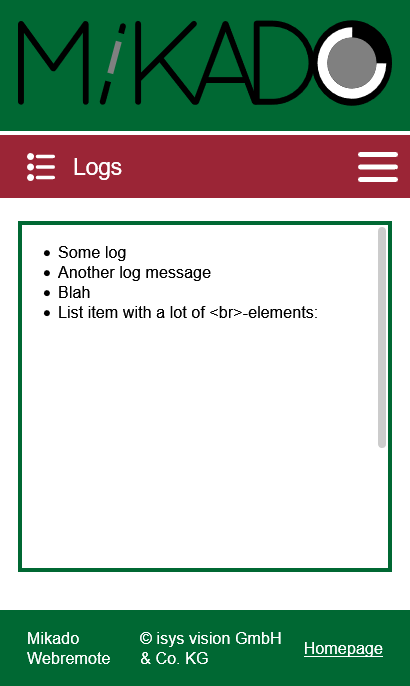
\includegraphics[width=\textwidth]{media/webremote-logs.png}
			\caption{Logfenster}
			\label{fig:webremote-logfenster}
		\end{minipage}
		\begin{minipage}{0.3\textwidth}
			\centering
			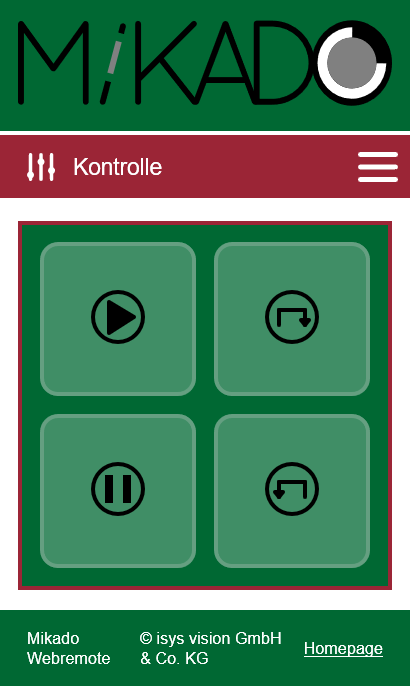
\includegraphics[width=\textwidth]{media/webremote-kontrolle.png}
			\caption{Kontrolle}
			\label{fig:webremote-kontrolle}
		\end{minipage}
		\begin{minipage}{0.3\textwidth}
			\centering
			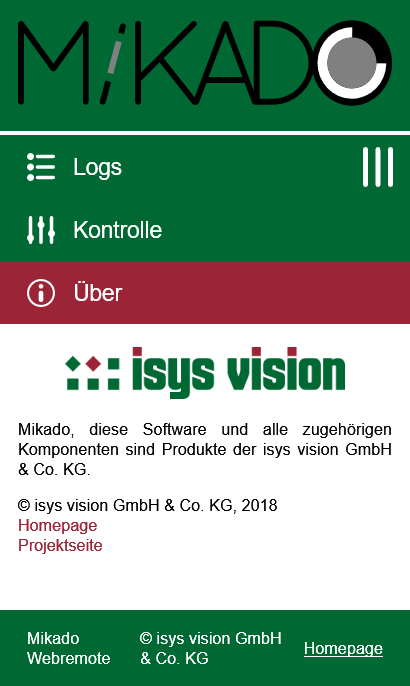
\includegraphics[width=\textwidth]{media/webremote-info.png}
			\caption{Info / Menü}
			\label{fig:webremote-info}
		\end{minipage}
	\end{center}
\end{figure}


\subsection{Befehls- und Logübertragung mithilfe von RosJS}

Auf dem Hostrechner des Roboters läuft zur Kontrolle von diesem eine Python-Bibliothek
namens ROS (Roboter Operating System). Sie bietet viele Funktionalitäten, beispielsweise
zum Steuern der einzelnen Gelenkwinkel durch Python.

Weiterhin werden Services zur Ausführung von einzelnen Aufgaben bereitgestellt.
Der Service \texttt{/reset} setzt beispielsweise den aktuellen Programmablauf
zurück und kann mit \texttt{rosservice call /reset} aufgerufen werden. Es sind
außerdem die Services \texttt{/run} und \texttt{/pause} vorhanden, welche die für
mich notwendige Funktionalität beinhalten. Die beiden letzteren werden mit Parametern
aufgerufen: \texttt{rosservice call /run ``step:false blocking:false''}, bzw.
\texttt{rosservice call /pause ``blocking:false''}.

Der Parameter \texttt{blocking} ist dabei in meinem Fall irrelevant; umso interessanter
ist jedoch das Argument \texttt{step}: Ist es auf \texttt{false} gesetzt, läuft
das Programm beim Aufruf normal durch. Sobald der Service jedoch mit \texttt{step:true}
aufgerufen wird, wird nur ein Schritt im Programmablauf durchgeführt.

Zur Anbindung an das von mir entwickelte Webinterface habe ich nun die Bibliothek
RoslibJS verwendet, welche als Kommunikationsmodul für ROS fungiert. Hiermit können
entsprechende Aufrufe im Javascript festgelegt werden, um diese anschließend an
den Hostrechner zu senden und somit den zugehörigen Service zu starten.

Meinen \texttt{<button>}-Elementen hatte ich jeweils die zugehörige Funktion im
Argument \texttt{onclick} zugeordnet (Beispiel: \texttt{<button onclick=''pause()''>Pause</button>}).
Im zugehörigen Javascript sind nun einmal die generelle Einrichtung von RoslibJS
(wie z.B. Verbindungsinformationen etc.) und für jeden Button die zugehörige Funktion
vorhanden.

\begin{code}[language=javascript, caption={Serviceaufruf durch RoslibJS}]
var ros = new ROSLIB.Ros();
ros.on('error', function(error) {/* Log weggelassen */});
ros.on('connection', function() {});
ros.on('close', function(){});
ros.connect('ws://10.0.4.136:8080');
/* Irrelevante Funktionen weggelassen */
function start() {
	var rosStart = new ROSLIB.Service({
		ros: ros,
		name: '/run',
		messageType: 'mikado_msgs/Run',
	});
	var rosStartRequest = new ROSLIB.ServiceRequest({
		step: false,
		blocking: false,
	});
	rosStart.callService(rosStartRequest);
}
/* Funktionsrumpf weggelassen */
function step() {};
function pause() {};
function reset() {};
/* Funktion zum Anhängen von Logs an das Logfenster. */
function addLog(messageText) {
	$('.log-window ul').append('<li>' + messageText + '</li>');
}
\end{code}

Zunächst wird in den ersten 5 Zeilen die Verbindung zum ROS hergestellt. In den
anschließend folgenden Funktionen wird zunächst ein neuer Service für die aktuelle
Routine erstellt (Zeilen 8 - 12), welcher dann mit einer Anfrage (Zeilen 13 - 16)
gestartet wird (Zeile 17). Der Service selbst enthält hierbei Informationen über
den aufgerufenen Befehl (in diesem Fall \texttt{/run}), während die Anfrage Informationen
über die Parameter enthält (hier die Argumente \texttt{step} und \texttt{blocking}).

Die Funktion \texttt{addLog(messageText)} in Zeile 24 bietet ein Interface, um neue
Lognachrichten ans Logfenster anzuhängen. Dazu wird der Logtext einfach als Listeneintrag
zur bestehenden Liste hinzugefügt.


\subsection{Webhosting und Netzwerk}

Nachdem das Interface nun eigentlich die gewünschte Funktionalität besitzt, muss
es noch erreichbar gemacht werden. Dazu wird ein HTTP-Server verwendet, welcher
die Webseite hostet. Mit der Python-Bibliothek \texttt{flask} ist dies recht einfach
zu realisieren:

\begin{code}[language=python, caption={Python-Skript zum Hosten des Webservers}]
import rospy
from flask import Flask, render_template
app = Flask(__name__)

@app.route('/')
def render_static():
    return render_template('index.html')
if __name__ == '__main__':
    app.run()
\end{code}

Nun lässt sich unter der IP-Adresse des Rechners (lokal \texttt{127.0.0.1}) die
gehostete Webseite aufrufen. Über ein WLAN-Netzwerk lässt sich nun eine Verbindung
zu mobilen Endgeräten aufbauen, welche dann auf das Webinterface zugreifen und somit
den Roboter kontrollieren können.



\section{Web-Preview zur Darstellung von Punktwolken}


